\section{Results}
The new simulation reproduces the measurements documented in \cite{2021-A549-model} accurately (cf. \Cref{figure:full-simulation-current,figure:simulation-error}, the remaining five cell cycle phase \& voltage protocol configurations were ommitted in this paper but can be verified via the online dashboard).
The simulation itself is accessible via its code interface, available from GitHub\footnote{\url{https://github.com/MrP01/InSilicoCancerCell}} and the live simulation dashboard.
Our method offers a set of significant numerical improvements in terms of the simulation runtime and optimization procedure, as presented in the previous chapter.

\begin{figure}[ht]
  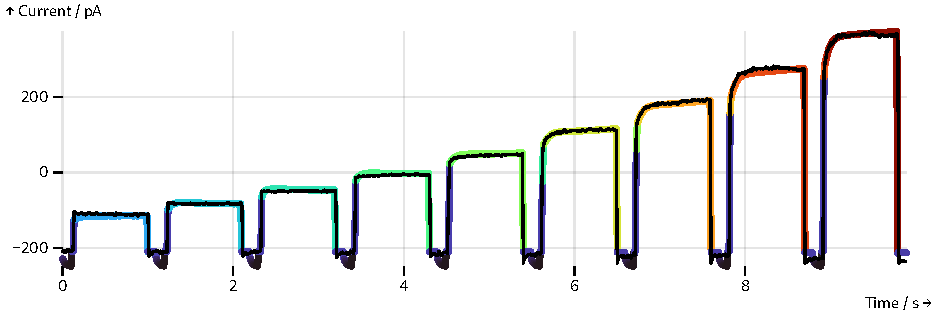
\includegraphics[width=\columnwidth]{../figures/results/full-simulation-current.pdf}
  \caption{The simulated and measured current response $I(t)$ across the membrane of an A549 cancer cell, given the \textit{activation} voltage protocol $V(t)$ in \Cref{figure:voltage-protocol}, recorded in the G0 phase of the cell cycle.}
  \label{figure:full-simulation-current}
\end{figure}
\begin{figure}
  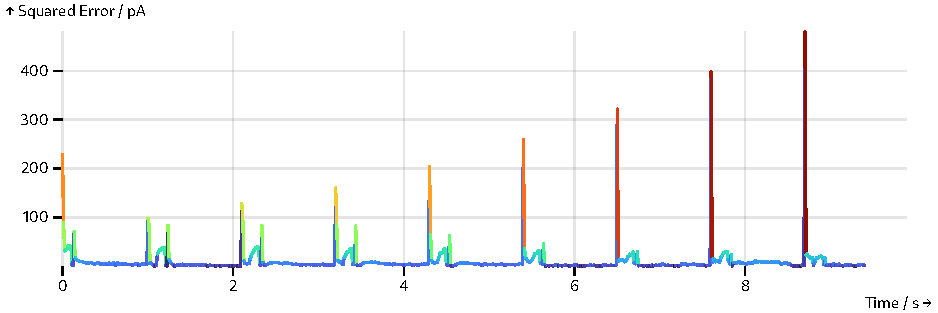
\includegraphics[width=\columnwidth]{../figures/results/simulation-error.pdf}
  \caption{Pointwise error between the measured current $\vec{I}_{\rm meas}$ and the simulated current $\vec{I}$, showing potential systematic problems within the computational model's representation of the ion channels as compared to the experimental results.}
  \label{figure:simulation-error}
\end{figure}

\subsection{Adaptive Timestepping}
With the standard forward iteration approach, the simulation takes 412 million steps to simulate over all voltage protocols and cell cycle phases, while the adaptive timestepping only requires 9 million steps for the same configuration.
While keeping the same level of accuracy when matching with the experimental data, our adaptive timestepping method is therefore 45 times faster than the standard approach, on average.
The time increment $\Delta t$ chosen at each point in the simulation can be found in \Cref{figure:dt-plot}.

\begin{figure}
  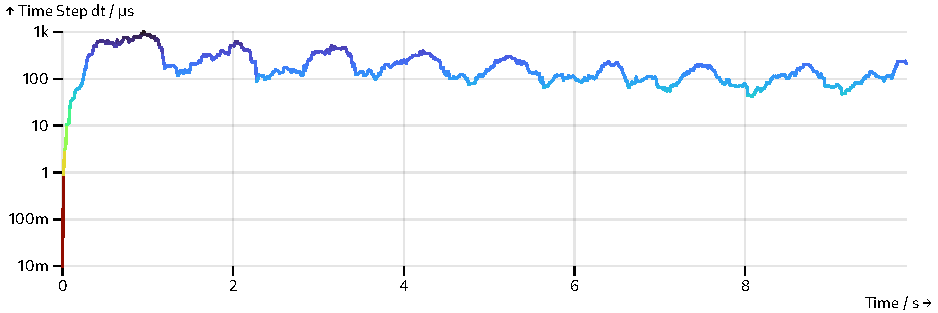
\includegraphics[width=\columnwidth]{../figures/results/dt-plot.pdf}
  \caption{Timestep $\Delta t$ throughout the duration of the simulation. $(\Delta t)_n$ is chosen in between simulation steps based on the heuristic given in \Cref{eq:dt-heuristic}. Red areas (small dt) indicate a high resolution within the simulation, blue areas indicate lower resolution (and therefore higher simulation speed).}
  \label{figure:dt-plot}
\end{figure}

In order to quantitatively establish the best possible state change tolerance $\Delta^{\rm tol}$, we recorded a number of simulation snapshots across different values for $\Delta^{\rm tol}$.
The results of this numerical experiment are documented in \Cref{figure:delta-tolerance}, which proves $\Delta^{\rm tol} = 10^{-4}$ to be the best choice.

\begin{figure}
  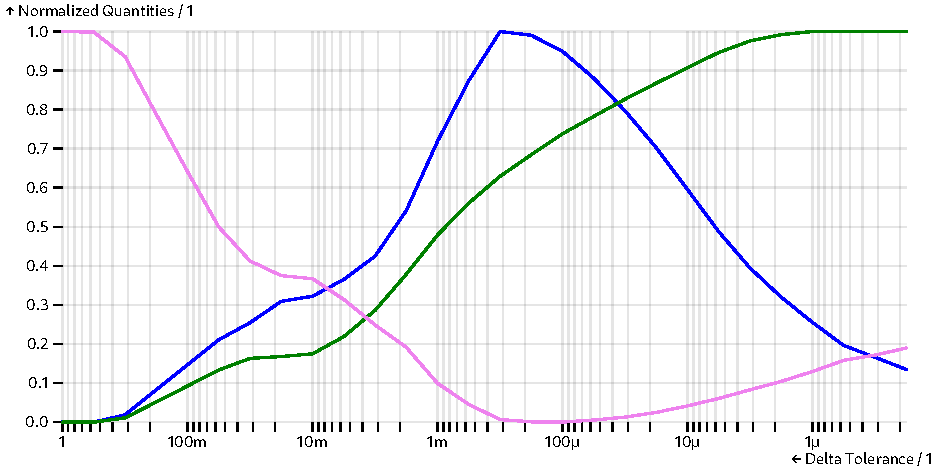
\includegraphics[width=\columnwidth]{../figures/results/delta-tolerance.pdf}
  \caption{Relative change of the average timestep $\Delta t$ (in blue), simulation runtime (in violet) and step acceptance rate (in green) when varying the delta tolerance $\Delta^{\rm tol}$ on a log-scale. All three quantities were normalized from their individual extent to $[0, 1]$. The most effective $\Delta^{\rm tol}$ is arguably on the order of $10^{-4}$.}
  \label{figure:delta-tolerance}
\end{figure}

\subsection{Inverse Problem}
We compare different optimization approaches based on their runtime and root mean square error,
$$\Delta_{\rm RMS} = \sqrt{\sfrac{1}{N_t} {\textstyle \sum_{j=1}^{N_t}} (I_j - I_{{\rm meas}, j})^2} = \frac{\norm{\vec{I} - \vec{I}_{\rm meas}}}{\sqrt{N_t}}\,.$$

\begin{table*}[ht]
  \centering
  \caption{Comparison of Optimization Approaches, evaluated on the G0 cell cycle phase with the activation voltage protocol (cf. \Cref{figure:voltage-protocol}). Runtime estimates were obtained on an Intel\texttrademark i7-5600U CPU.}
  \begin{tabular}{llrr}
    \textbf{Algorithm}                          & \textbf{Abbreviation} & \textbf{Runtime} / ms & \textbf{RMSE} / pA \\
    \midrule
    Particle Swarm Optimization                 & PSO                   & 22571                 & 27.69              \\
    Gradient Descent + More Thuente             & GD                    & 18924                 & 32.34              \\
    Limited-Memory BFGS + Hager Zhang           & LBFGS                 & 4845                  & 32.20              \\
    Non-Negative Least Squares \cite{1997-nnls} & NNLS                  & 318                   & 28.00              \\
    Quadratic Program                           & QP                    & 18                    & 28.13              \\
  \end{tabular}
  \label{table:optimization-comparison}
\end{table*}

Specifically, the best performing formulation for the channel counts problem in this context is the Quadratic Program (QP), cf. \Cref{table:optimization-comparison}.
The program was solved using the Clarabel \parencite{2024-clarabel} optimization library (also written in Rust), which completes the procedure in just 18 milliseconds.
Measurements and simulation were compared based on an FFT-accelerated Gauss-kernel convolution smoothed version of the 180,000 point measurements.

\subsection{Live Simulation Dashboard}
A screenshot of the simulation environment built upon the methods described in this paper is documented in \Cref{figure:screenshot}.

\begin{figure*}[ht]
  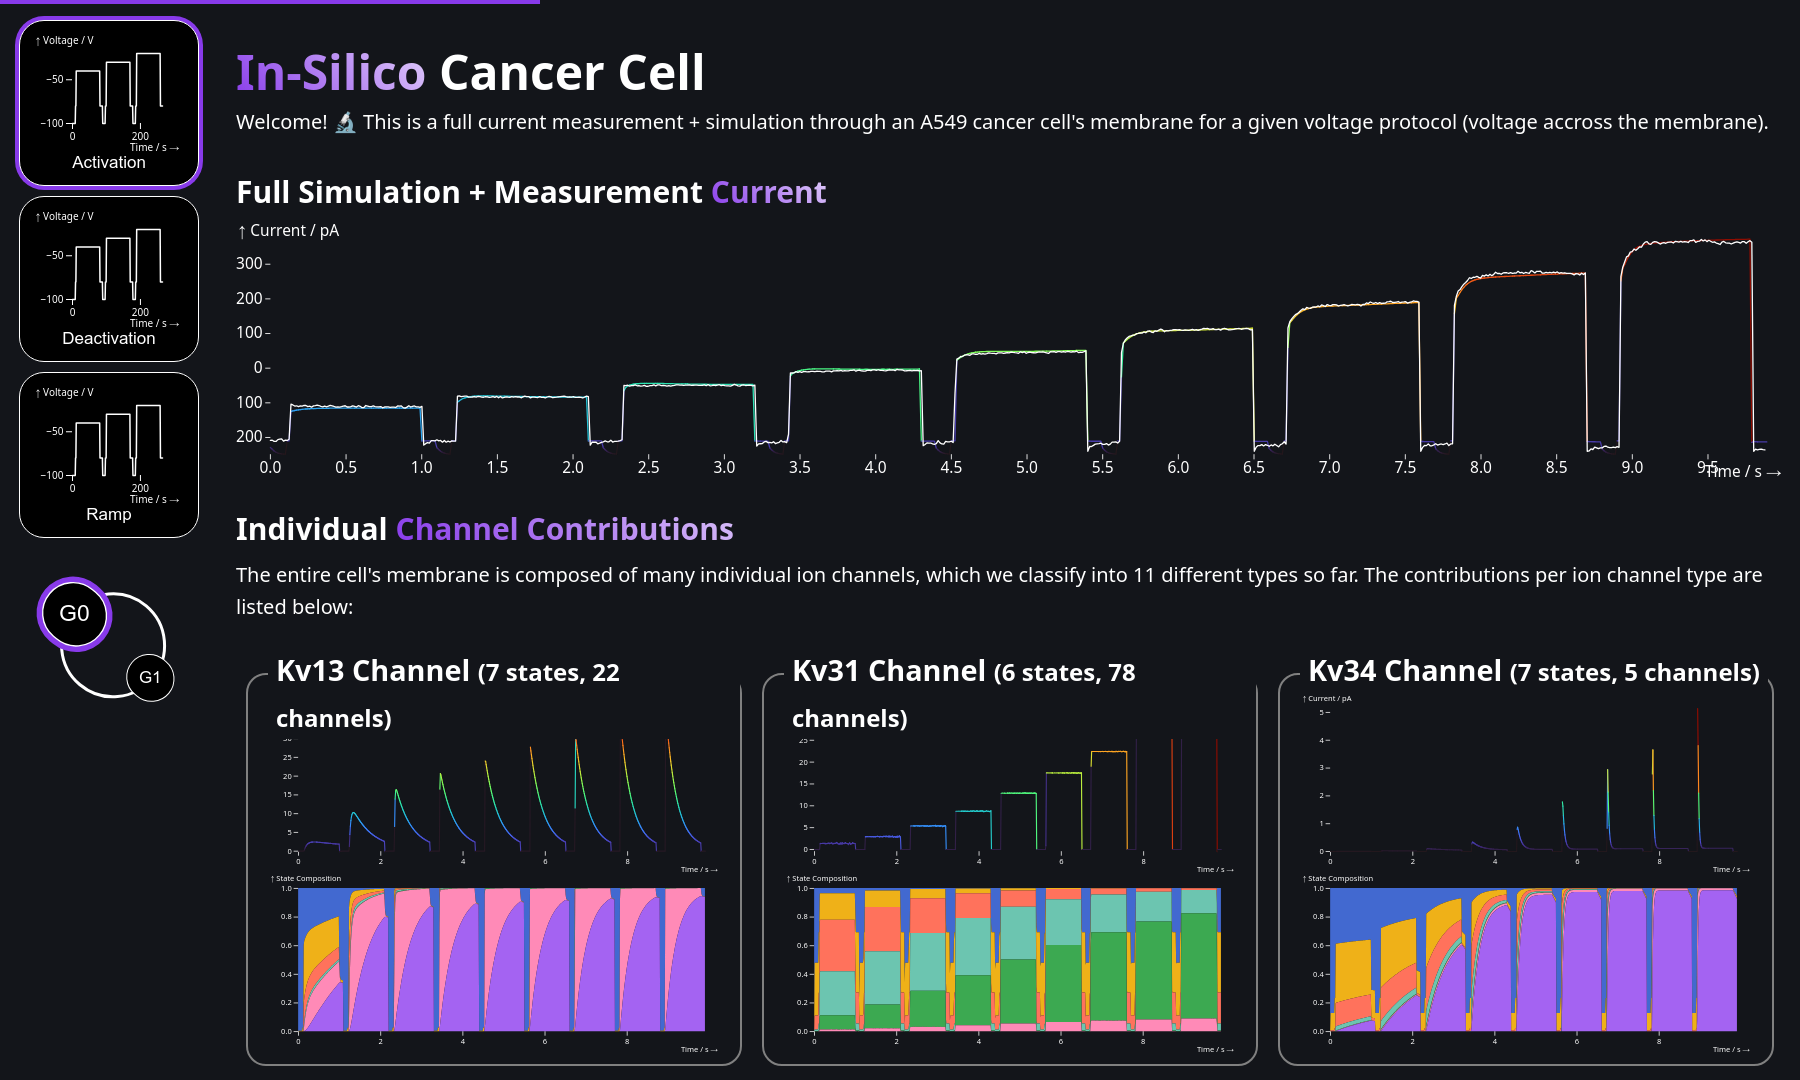
\includegraphics[width=\textwidth]{../figures/above-the-fold-screenshot.png}
  \caption{Screenshot of the live simulation dashboard, available here: \url{https://in-silico.hce.tugraz.at/}. This is the graphical user interface to the simulation written in Rust. The full simulation, completing within around 500ms, runs live in the browser using Rust's bindings to WebAssembly. One can choose the voltage protocol and cell cycle phase (G0/G1) in the menu on the left, while the full current and individual channel currents and internal states can be seen on the right. The remaining ion channel types have been cut off on this screenshot.}
  \label{figure:screenshot}
\end{figure*}
